\documentclass[12pt,a4paper]{article}
\usepackage[utf8]{vietnam}
\usepackage{amsmath,amssymb}
\usepackage{tabularx}
\usepackage{tikz}
\usepackage{xcolor}
\usepackage[top=0.6cm, bottom=0.6cm, left=0.6cm, right=0.6cm]{geometry}
\usepackage[dethi]{ex_test}

\SAOPTN{widthSA=2.6,heightSA=0.62}
\setlength{\parskip}{0pt}

% Dong ke cham mo chuan viet tay
\newcommand{\dongke}[1]{%
  \begingroup%
  \setlength{\parskip}{0pt}%
  \baselineskip=18.5pt%
  \vspace{1.0mm}%
  \foreach \i in {1,...,#1}{%
    \noindent{\color{gray!60}\dotfill}\par%
  }%
  \vspace{0.6mm}%
  \endgroup%
}

% Khu vuc bai lam chia 2 cot co vach ngan mo o giua
\newcommand{\dongkeHaiCot}[1]{%
  \par\vspace{0.5mm}%
  \noindent%
  \begin{minipage}[t]{0.485\linewidth}%
    \dongke{#1}%
  \end{minipage}%
  \hfill%
  {\color{gray!60}\vrule}%
  \hfill%
  \begin{minipage}[t]{0.485\linewidth}%
    \dongke{#1}%
  \end{minipage}%
}

% Dinh nghia o bai tap tu luan trong bang
\newcommand{\oBaiTap}[3][5]{%
  \vspace{1.0mm}%
  \noindent\textbf{#2} #3\par%
  \dongke{#1}%
}

\begin{document}
\pagestyle{empty}
% =============================================================================
% ========================= TOAN 7 TUAN 10 BUOI 01 - MA DE 101 =================
% ========================= TRANG 1/2 ==========================================
% =============================================================================
\noindent
\begin{tabularx}{\linewidth}{|X|c|}
\hline
\textbf{PHIẾU KIỂM TRA ĐỊNH KỲ TOÁN 7 - TUẦN 10 - BUỔI 01} & \textbf{Mã đề: 101 - Trang 1/2} \\
\hline
\end{tabularx}

\vspace{1.2mm}

\noindent
\begin{tabularx}{\linewidth}{|p{3.2cm}|X|}
\hline
\centering\textbf{ĐIỂM SỐ} & \centering\textbf{LỜI NHẬN XÉT CỦA THẦY CÔ} \tabularnewline
\hline
\rule{0pt}{1.8cm} & \tabularnewline
\hline
\end{tabularx}

\vspace{1.5mm}
\noindent\textbf{Câu 1 (0,25 điểm).} Số đối của số hữu tỉ $-\dfrac{5}{7}$ là: \shortans{\dfrac{5}{7}}\par\vspace{2.3mm}
\noindent\textbf{Câu 2 (0,25 điểm).} Giá trị của căn bậc hai số học $\sqrt{49}$ bằng: \shortans{7}\par\vspace{2.3mm}
\noindent\textbf{Câu 3 (0,25 điểm).} Giá trị của biểu thức $|-5{,}35|$ bằng: \shortans{5{,}35}\par\vspace{2.3mm}
\noindent\textbf{Câu 4 (0,25 điểm).} Cho $\Delta ABC = \Delta MNP$. Đỉnh tương ứng với đỉnh $B$ là: \shortans{\text{Đỉnh } N}\par\vspace{2.3mm}
\noindent\textbf{Câu 5 (0,25 điểm).} Cho $\Delta ABC = \Delta DEF$, biết $AB = 6\text{ cm}$. Độ dài cạnh $DE$ là: \shortans{6\text{ cm}}\par\vspace{2.3mm}
\noindent\textbf{Câu 6 (0,25 điểm).} Cho $\Delta ABC = \Delta MNP$, có $\widehat{A} = 65^\circ, \widehat{B} = 55^\circ$. Số đo góc $\widehat{P}$ là: \shortans{60^\circ}\par\vspace{2.3mm}
\noindent\textbf{Câu 7 (0,25 điểm).} Cho $\Delta ABC = \Delta DEF$. Biết chu vi $\Delta ABC$ bằng $26\text{ cm}$. Chu vi $\Delta DEF$ là: \shortans{26\text{ cm}}\par\vspace{2.3mm}
\noindent\textbf{Câu 8 (0,25 điểm).} Để $\Delta ABC = \Delta MNP$ (c.c.c) khi có $AB=MN, BC=NP$, cần thêm: \shortans{AC = MP}\par\vspace{2.3mm}
\noindent\textbf{Câu 9 (0,25 điểm).} Cho đoạn $AB$, có $AC = AD, BC = BD$. Cạnh chung của $\Delta ABC, \Delta ABD$ là: \shortans{\text{Cạnh } AB}\par\vspace{2.3mm}
\noindent\textbf{Câu 10 (0,25 điểm).} Các thanh ghép thành hình tam giác trong giàn giáo xây dựng giúp kết cấu: \shortans{\text{Cứng vững}}\par\vspace{2.3mm}
\vspace{0.2mm}
\noindent\textbf{Câu 11 (3,0 điểm). Thực hiện phép tính (hợp lý nếu có thể):}
\vspace{0.8mm}

\noindent
\begin{tabularx}{\linewidth}{|X|X|}
\hline
\oBaiTap[5]{a) (0,5 điểm)}{$\dfrac{5}{8} + \dfrac{7}{16} - \dfrac{1}{2}$} & 
\oBaiTap[5]{b) (0,5 điểm)}{$\dfrac{5}{11} \cdot \left(-\dfrac{4}{7}\right) + \dfrac{5}{11} \cdot \left(-\dfrac{3}{7}\right)$} \\
\hline
\oBaiTap[5]{c) (0,5 điểm)}{$\left(-\dfrac{1}{2}\right)^3 : \dfrac{1}{8} + \dfrac{2}{5} \cdot 5$} & 
\oBaiTap[5]{d) (0,5 điểm)}{$\sqrt{\dfrac{49}{25}} - \left|-\dfrac{2}{5}\right| + \dfrac{3}{5}$} \\
\hline
\oBaiTap[5]{e) (0,5 điểm)}{$\dfrac{7}{3} - \left[\dfrac{2}{3} + \left(\dfrac{1}{2}\right)^2 \cdot 4\right]$} & 
\oBaiTap[5]{f) (0,5 điểm)}{$\dfrac{2^{12} \cdot 9^4}{4^5 \cdot 3^7}$} \\
\hline
\end{tabularx}

\newpage
% =============================================================================
% ========================= TOAN 7 TUAN 10 BUOI 01 - MA DE 101 =================
% ========================= TRANG 2/2 ==========================================
% =============================================================================
\noindent
\begin{tabularx}{\linewidth}{|X|c|}
\hline
\textbf{TOÁN 7 - TUẦN 10 - BUỔI 01} & \textbf{Mã đề: 101 - Trang 2/2} \\
\hline
\end{tabularx}

\vspace{1.5mm}

\noindent\textbf{Câu 12 (2,0 điểm). Tìm số hữu tỉ $x$, biết:}
\vspace{0.8mm}

\noindent
\begin{tabularx}{\linewidth}{|X|X|}
\hline
\oBaiTap[5]{a) (0,5 điểm)}{$x - \dfrac{2}{5} = \dfrac{7}{10}$} & 
\oBaiTap[5]{b) (0,5 điểm)}{$\dfrac{3}{4}x + \dfrac{1}{2} = \dfrac{7}{8}$} \\
\hline
\oBaiTap[5]{c) (0,5 điểm)}{$\left(x - \dfrac{1}{2}\right)^2 = \dfrac{9}{25}$} & 
\oBaiTap[5]{d) (0,5 điểm)}{$\left|2x - \dfrac{1}{3}\right| = \dfrac{5}{3}$} \\
\hline
\end{tabularx}

\vspace{1.5mm}

\noindent
\begin{tabularx}{\linewidth}{|X|}
\hline
\vspace{0.5mm}
\begin{minipage}[t]{0.68\linewidth}
\vspace{0pt}
\textbf{Câu 13 (2,0 điểm).} Cho góc nhọn $\widehat{xOy}$. Trên tia $Ox$ lấy điểm $A$, trên tia $Oy$ lấy điểm $B$ sao cho $OA = OB$. Lấy điểm $C$ nằm bên trong góc $\widehat{xOy}$ sao cho $AC = BC$.\par\vspace{0.4mm}
\textbf{a)} (1,0 điểm) Chứng minh rằng $\Delta OAC = \Delta OBC$.\par\vspace{0.4mm}
\textbf{b)} (1,0 điểm) Chứng minh rằng $OC$ là tia phân giác của góc $\widehat{xOy}$. Biết $\widehat{xOy} = 70^\circ$, tính số đo góc $\widehat{AOC}$.
\end{minipage}\hfill
\begin{minipage}[t]{0.30\linewidth}
\vspace{0pt}\centering
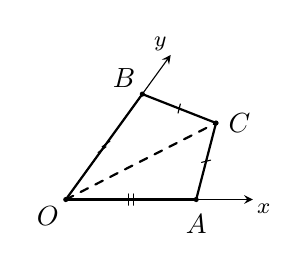
\begin{tikzpicture}[scale=0.72, >=stealth, line join=round, line cap=round]
  \coordinate (O) at (0, 0);
  \coordinate (X) at (3.3, 0);
  \coordinate (Y) at (1.85, 2.55);
  \coordinate (A) at (2.3, 0);
  \coordinate (B) at (1.35, 1.86);
  \coordinate (C) at (2.65, 1.35);

  % Tia Ox, Oy
  \draw[->] (O) -- (X) node[below right=-2pt] {\footnotesize $x$};
  \draw[->] (O) -- (Y) node[above left=-2pt] {\footnotesize $y$};

  % Cac doan thang
  \draw[thick] (O) -- (A);
  \draw[thick] (O) -- (B);
  \draw[thick] (A) -- (C);
  \draw[thick] (B) -- (C);
  \draw[thick, dashed] (O) -- (C);

  % Vach danh dau bang nhau OA = OB (2 vach cat ngang)
  \draw (1.1, -0.1) -- (1.1, 0.1);
  \draw (1.2, -0.1) -- (1.2, 0.1);
  \draw (0.64 - 0.07, 0.88 - 0.05) -- (0.64 + 0.07, 0.88 + 0.05);
  \draw (0.71 - 0.07, 0.98 - 0.05) -- (0.71 + 0.07, 0.98 + 0.05);

  % Vach danh dau bang nhau AC = BC (1 vach cat ngang)
  \draw (2.475 - 0.08, 0.675 - 0.02) -- (2.475 + 0.08, 0.675 + 0.02);
  \draw (2.0 - 0.02, 1.605 - 0.08) -- (2.0 + 0.02, 1.605 + 0.08);

  % Cac diem va nhan
  \fill (O) circle (1.3pt) node[below left=-1pt] {$O$};
  \fill (A) circle (1.3pt) node[below=2pt] {$A$};
  \fill (B) circle (1.3pt) node[above left=-1pt] {$B$};
  \fill (C) circle (1.3pt) node[right=1pt] {$C$};
\end{tikzpicture}
\end{minipage}\par
\vspace{0.4mm}
\noindent\textit{Bài giải:}\dongkeHaiCot{10}
\\ \hline
\end{tabularx}

\vspace{1.5mm}

\noindent
\begin{tabularx}{\linewidth}{|X|}
\hline
\vspace{0.5mm}
\textbf{Câu 14 (0,5 điểm).} Tìm giá trị nhỏ nhất của biểu thức: $A = |x - 2026| + |x - 10|$.\par
\vspace{0.4mm}
\noindent\textit{Bài giải:}\dongkeHaiCot{6}
\\ \hline
\end{tabularx}

\newpage
% =============================================================================
% ========================= TOAN 7 TUAN 10 BUOI 01 - MA DE 102 =================
% ========================= TRANG 1/2 ==========================================
% =============================================================================
\noindent
\begin{tabularx}{\linewidth}{|X|c|}
\hline
\textbf{PHIẾU KIỂM TRA ĐỊNH KỲ TOÁN 7 - TUẦN 10 - BUỔI 01} & \textbf{Mã đề: 102 - Trang 1/2} \\
\hline
\end{tabularx}

\vspace{1.2mm}

\noindent
\begin{tabularx}{\linewidth}{|p{3.2cm}|X|}
\hline
\centering\textbf{ĐIỂM SỐ} & \centering\textbf{LỜI NHẬN XÉT CỦA THẦY CÔ} \tabularnewline
\hline
\rule{0pt}{1.8cm} & \tabularnewline
\hline
\end{tabularx}

\vspace{1.5mm}
\noindent\textbf{Câu 1 (0,25 điểm).} Số đối của số hữu tỉ $-\dfrac{3}{8}$ là: \shortans{\dfrac{3}{8}}\par\vspace{2.3mm}
\noindent\textbf{Câu 2 (0,25 điểm).} Giá trị của căn bậc hai số học $\sqrt{64}$ bằng: \shortans{8}\par\vspace{2.3mm}
\noindent\textbf{Câu 3 (0,25 điểm).} Giá trị của biểu thức $|-6{,}45|$ bằng: \shortans{6{,}45}\par\vspace{2.3mm}
\noindent\textbf{Câu 4 (0,25 điểm).} Cho $\Delta DEF = \Delta MNP$. Đỉnh tương ứng với đỉnh $F$ là: \shortans{\text{Đỉnh } P}\par\vspace{2.3mm}
\noindent\textbf{Câu 5 (0,25 điểm).} Cho $\Delta MNP = \Delta QRS$, biết $NP = 7\text{ cm}$. Độ dài cạnh $RS$ là: \shortans{7\text{ cm}}\par\vspace{2.3mm}
\noindent\textbf{Câu 6 (0,25 điểm).} Cho $\Delta ABC = \Delta DEF$, có $\widehat{A} = 70^\circ, \widehat{B} = 45^\circ$. Số đo góc $\widehat{F}$ là: \shortans{65^\circ}\par\vspace{2.3mm}
\noindent\textbf{Câu 7 (0,25 điểm).} Cho $\Delta MNP = \Delta GHK$. Biết chu vi $\Delta MNP$ bằng $32\text{ cm}$. Chu vi $\Delta GHK$ là: \shortans{32\text{ cm}}\par\vspace{2.3mm}
\noindent\textbf{Câu 8 (0,25 điểm).} Để $\Delta DEF = \Delta GHK$ (c.c.c) khi có $DE=GH, DF=GK$, cần thêm: \shortans{EF = HK}\par\vspace{2.3mm}
\noindent\textbf{Câu 9 (0,25 điểm).} Cho đoạn $MN$, có $MP = MQ, NP = NQ$. Cạnh chung của $\Delta MNP, \Delta MNQ$ là: \shortans{\text{Cạnh } MN}\par\vspace{2.3mm}
\noindent\textbf{Câu 10 (0,25 điểm).} Chân máy ảnh (tripod) luôn đứng vững vì ba chân tạo với mặt đất một: \shortans{\text{Hình tam giác}}\par\vspace{2.3mm}
\vspace{0.2mm}
\noindent\textbf{Câu 11 (3,0 điểm). Thực hiện phép tính (hợp lý nếu có thể):}
\vspace{0.8mm}

\noindent
\begin{tabularx}{\linewidth}{|X|X|}
\hline
\oBaiTap[5]{a) (0,5 điểm)}{$\dfrac{3}{7} + \dfrac{9}{14} - \dfrac{1}{2}$} & 
\oBaiTap[5]{b) (0,5 điểm)}{$\dfrac{4}{9} \cdot \left(-\dfrac{5}{8}\right) + \dfrac{4}{9} \cdot \left(-\dfrac{3}{8}\right)$} \\
\hline
\oBaiTap[5]{c) (0,5 điểm)}{$\left(-\dfrac{1}{3}\right)^2 \cdot 18 - \dfrac{4}{7} : \dfrac{2}{7}$} & 
\oBaiTap[5]{d) (0,5 điểm)}{$\sqrt{\dfrac{36}{49}} - \left|-\dfrac{2}{7}\right| + \dfrac{5}{7}$} \\
\hline
\oBaiTap[5]{e) (0,5 điểm)}{$\dfrac{8}{3} - \left[\dfrac{1}{3} + \left(\dfrac{1}{3}\right)^2 \cdot 9\right]$} & 
\oBaiTap[5]{f) (0,5 điểm)}{$\dfrac{3^{11} \cdot 4^4}{9^5 \cdot 2^6}$} \\
\hline
\end{tabularx}

\newpage
% =============================================================================
% ========================= TOAN 7 TUAN 10 BUOI 01 - MA DE 102 =================
% ========================= TRANG 2/2 ==========================================
% =============================================================================
\noindent
\begin{tabularx}{\linewidth}{|X|c|}
\hline
\textbf{TOÁN 7 - TUẦN 10 - BUỔI 01} & \textbf{Mã đề: 102 - Trang 2/2} \\
\hline
\end{tabularx}

\vspace{1.5mm}

\noindent\textbf{Câu 12 (2,0 điểm). Tìm số hữu tỉ $x$, biết:}
\vspace{0.8mm}

\noindent
\begin{tabularx}{\linewidth}{|X|X|}
\hline
\oBaiTap[5]{a) (0,5 điểm)}{$x - \dfrac{3}{4} = \dfrac{5}{8}$} & 
\oBaiTap[5]{b) (0,5 điểm)}{$\dfrac{2}{5}x + \dfrac{1}{3} = \dfrac{11}{15}$} \\
\hline
\oBaiTap[5]{c) (0,5 điểm)}{$\left(x - \dfrac{1}{3}\right)^2 = \dfrac{16}{25}$} & 
\oBaiTap[5]{d) (0,5 điểm)}{$\left|3x - \dfrac{1}{2}\right| = \dfrac{5}{2}$} \\
\hline
\end{tabularx}

\vspace{1.5mm}

\noindent
\begin{tabularx}{\linewidth}{|X|}
\hline
\vspace{0.5mm}
\begin{minipage}[t]{0.68\linewidth}
\vspace{0pt}
\textbf{Câu 13 (2,0 điểm).} Cho góc nhọn $\widehat{xOy}$. Trên tia $Ox$ lấy điểm $A$, trên tia $Oy$ lấy điểm $B$ sao cho $OA = OB$. Lấy điểm $C$ nằm bên trong góc $\widehat{xOy}$ sao cho $AC = BC$.\par\vspace{0.4mm}
\textbf{a)} (1,0 điểm) Chứng minh rằng $\Delta OAC = \Delta OBC$.\par\vspace{0.4mm}
\textbf{b)} (1,0 điểm) Chứng minh rằng $OC$ là tia phân giác của góc $\widehat{xOy}$. Biết $\widehat{xOy} = 80^\circ$, tính số đo góc $\widehat{AOC}$.
\end{minipage}\hfill
\begin{minipage}[t]{0.30\linewidth}
\vspace{0pt}\centering
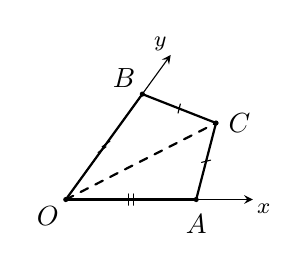
\begin{tikzpicture}[scale=0.72, >=stealth, line join=round, line cap=round]
  \coordinate (O) at (0, 0);
  \coordinate (X) at (3.3, 0);
  \coordinate (Y) at (1.85, 2.55);
  \coordinate (A) at (2.3, 0);
  \coordinate (B) at (1.35, 1.86);
  \coordinate (C) at (2.65, 1.35);

  % Tia Ox, Oy
  \draw[->] (O) -- (X) node[below right=-2pt] {\footnotesize $x$};
  \draw[->] (O) -- (Y) node[above left=-2pt] {\footnotesize $y$};

  % Cac doan thang
  \draw[thick] (O) -- (A);
  \draw[thick] (O) -- (B);
  \draw[thick] (A) -- (C);
  \draw[thick] (B) -- (C);
  \draw[thick, dashed] (O) -- (C);

  % Vach danh dau bang nhau OA = OB (2 vach cat ngang)
  \draw (1.1, -0.1) -- (1.1, 0.1);
  \draw (1.2, -0.1) -- (1.2, 0.1);
  \draw (0.64 - 0.07, 0.88 - 0.05) -- (0.64 + 0.07, 0.88 + 0.05);
  \draw (0.71 - 0.07, 0.98 - 0.05) -- (0.71 + 0.07, 0.98 + 0.05);

  % Vach danh dau bang nhau AC = BC (1 vach cat ngang)
  \draw (2.475 - 0.08, 0.675 - 0.02) -- (2.475 + 0.08, 0.675 + 0.02);
  \draw (2.0 - 0.02, 1.605 - 0.08) -- (2.0 + 0.02, 1.605 + 0.08);

  % Cac diem va nhan
  \fill (O) circle (1.3pt) node[below left=-1pt] {$O$};
  \fill (A) circle (1.3pt) node[below=2pt] {$A$};
  \fill (B) circle (1.3pt) node[above left=-1pt] {$B$};
  \fill (C) circle (1.3pt) node[right=1pt] {$C$};
\end{tikzpicture}
\end{minipage}\par
\vspace{0.4mm}
\noindent\textit{Bài giải:}\dongkeHaiCot{10}
\\ \hline
\end{tabularx}

\vspace{1.5mm}

\noindent
\begin{tabularx}{\linewidth}{|X|}
\hline
\vspace{0.5mm}
\textbf{Câu 14 (0,5 điểm).} Tìm giá trị nhỏ nhất của biểu thức: $A = |x - 2025| + |x - 15|$.\par
\vspace{0.4mm}
\noindent\textit{Bài giải:}\dongkeHaiCot{6}
\\ \hline
\end{tabularx}

\newpage
% =============================================================================
% ========================= TOAN 7 TUAN 10 BUOI 01 - MA DE 103 =================
% ========================= TRANG 1/2 ==========================================
% =============================================================================
\noindent
\begin{tabularx}{\linewidth}{|X|c|}
\hline
\textbf{PHIẾU KIỂM TRA ĐỊNH KỲ TOÁN 7 - TUẦN 10 - BUỔI 01} & \textbf{Mã đề: 103 - Trang 1/2} \\
\hline
\end{tabularx}

\vspace{1.2mm}

\noindent
\begin{tabularx}{\linewidth}{|p{3.2cm}|X|}
\hline
\centering\textbf{ĐIỂM SỐ} & \centering\textbf{LỜI NHẬN XÉT CỦA THẦY CÔ} \tabularnewline
\hline
\rule{0pt}{1.8cm} & \tabularnewline
\hline
\end{tabularx}

\vspace{1.5mm}
\noindent\textbf{Câu 1 (0,25 điểm).} Số đối của số hữu tỉ $-\dfrac{4}{9}$ là: \shortans{\dfrac{4}{9}}\par\vspace{2.3mm}
\noindent\textbf{Câu 2 (0,25 điểm).} Giá trị của căn bậc hai số học $\sqrt{100}$ bằng: \shortans{10}\par\vspace{2.3mm}
\noindent\textbf{Câu 3 (0,25 điểm).} Giá trị của biểu thức $|-8{,}25|$ bằng: \shortans{8{,}25}\par\vspace{2.3mm}
\noindent\textbf{Câu 4 (0,25 điểm).} Cho $\Delta ABC = \Delta HIK$. Cạnh tương ứng với cạnh $AC$ là: \shortans{\text{Cạnh } HK}\par\vspace{2.3mm}
\noindent\textbf{Câu 5 (0,25 điểm).} Cho $\Delta ABC = \Delta MNP$, biết $AC = 5\text{ cm}$. Độ dài cạnh $MP$ là: \shortans{5\text{ cm}}\par\vspace{2.3mm}
\noindent\textbf{Câu 6 (0,25 điểm).} Cho $\Delta MNP = \Delta HIK$, có $\widehat{M} = 80^\circ, \widehat{N} = 40^\circ$. Số đo góc $\widehat{K}$ là: \shortans{60^\circ}\par\vspace{2.3mm}
\noindent\textbf{Câu 7 (0,25 điểm).} $\Delta ABC$ có ba cạnh $5, 7, 8\text{ cm}$. Nếu $\Delta ABC = \Delta DEF$ thì chu vi $\Delta DEF$ là: \shortans{20\text{ cm}}\par\vspace{2.3mm}
\noindent\textbf{Câu 8 (0,25 điểm).} Để $\Delta ABC = \Delta DEG$ (c.c.c) khi có $BC=EG, AC=DG$, cần thêm: \shortans{AB = DE}\par\vspace{2.3mm}
\noindent\textbf{Câu 9 (0,25 điểm).} Cho góc $\widehat{xOy}$ có $OA = OB, CA = CB$. Cạnh chung $\Delta OAC, \Delta OBC$ là: \shortans{\text{Cạnh } OC}\par\vspace{2.3mm}
\noindent\textbf{Câu 10 (0,25 điểm).} Đóng thêm thanh giằng chéo vào khung cửa sổ chữ nhật nhằm tạo thành các: \shortans{\text{Hình tam giác}}\par\vspace{2.3mm}
\vspace{0.2mm}
\noindent\textbf{Câu 11 (3,0 điểm). Thực hiện phép tính (hợp lý nếu có thể):}
\vspace{0.8mm}

\noindent
\begin{tabularx}{\linewidth}{|X|X|}
\hline
\oBaiTap[5]{a) (0,5 điểm)}{$\dfrac{5}{9} + \dfrac{7}{18} - \dfrac{1}{3}$} & 
\oBaiTap[5]{b) (0,5 điểm)}{$\dfrac{3}{10} \cdot \left(-\dfrac{4}{9}\right) + \dfrac{3}{10} \cdot \left(-\dfrac{5}{9}\right)$} \\
\hline
\oBaiTap[5]{c) (0,5 điểm)}{$\left(-\dfrac{1}{2}\right)^4 \cdot 32 - \dfrac{5}{6} : \dfrac{5}{12}$} & 
\oBaiTap[5]{d) (0,5 điểm)}{$\sqrt{\dfrac{64}{25}} - \left|-\dfrac{3}{5}\right| + \dfrac{2}{5}$} \\
\hline
\oBaiTap[5]{e) (0,5 điểm)}{$\dfrac{9}{4} - \left[\dfrac{3}{4} + \left(\dfrac{1}{2}\right)^3 \cdot 8\right]$} & 
\oBaiTap[5]{f) (0,5 điểm)}{$\dfrac{2^{10} \cdot 25^3}{10^5 \cdot 5}$} \\
\hline
\end{tabularx}

\newpage
% =============================================================================
% ========================= TOAN 7 TUAN 10 BUOI 01 - MA DE 103 =================
% ========================= TRANG 2/2 ==========================================
% =============================================================================
\noindent
\begin{tabularx}{\linewidth}{|X|c|}
\hline
\textbf{TOÁN 7 - TUẦN 10 - BUỔI 01} & \textbf{Mã đề: 103 - Trang 2/2} \\
\hline
\end{tabularx}

\vspace{1.5mm}

\noindent\textbf{Câu 12 (2,0 điểm). Tìm số hữu tỉ $x$, biết:}
\vspace{0.8mm}

\noindent
\begin{tabularx}{\linewidth}{|X|X|}
\hline
\oBaiTap[5]{a) (0,5 điểm)}{$x - \dfrac{4}{7} = \dfrac{3}{14}$} & 
\oBaiTap[5]{b) (0,5 điểm)}{$\dfrac{4}{5}x + \dfrac{1}{4} = \dfrac{13}{20}$} \\
\hline
\oBaiTap[5]{c) (0,5 điểm)}{$\left(x - \dfrac{2}{5}\right)^2 = \dfrac{9}{16}$} & 
\oBaiTap[5]{d) (0,5 điểm)}{$\left|2x - \dfrac{3}{4}\right| = \dfrac{5}{4}$} \\
\hline
\end{tabularx}

\vspace{1.5mm}

\noindent
\begin{tabularx}{\linewidth}{|X|}
\hline
\vspace{0.5mm}
\begin{minipage}[t]{0.68\linewidth}
\vspace{0pt}
\textbf{Câu 13 (2,0 điểm).} Cho góc nhọn $\widehat{xOy}$. Trên tia $Ox$ lấy điểm $A$, trên tia $Oy$ lấy điểm $B$ sao cho $OA = OB$. Lấy điểm $C$ nằm bên trong góc $\widehat{xOy}$ sao cho $AC = BC$.\par\vspace{0.4mm}
\textbf{a)} (1,0 điểm) Chứng minh rằng $\Delta OAC = \Delta OBC$.\par\vspace{0.4mm}
\textbf{b)} (1,0 điểm) Chứng minh rằng $OC$ là tia phân giác của góc $\widehat{xOy}$. Biết $\widehat{xOy} = 60^\circ$, tính số đo góc $\widehat{AOC}$.
\end{minipage}\hfill
\begin{minipage}[t]{0.30\linewidth}
\vspace{0pt}\centering
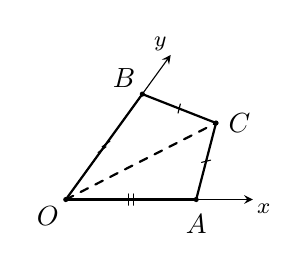
\begin{tikzpicture}[scale=0.72, >=stealth, line join=round, line cap=round]
  \coordinate (O) at (0, 0);
  \coordinate (X) at (3.3, 0);
  \coordinate (Y) at (1.85, 2.55);
  \coordinate (A) at (2.3, 0);
  \coordinate (B) at (1.35, 1.86);
  \coordinate (C) at (2.65, 1.35);

  % Tia Ox, Oy
  \draw[->] (O) -- (X) node[below right=-2pt] {\footnotesize $x$};
  \draw[->] (O) -- (Y) node[above left=-2pt] {\footnotesize $y$};

  % Cac doan thang
  \draw[thick] (O) -- (A);
  \draw[thick] (O) -- (B);
  \draw[thick] (A) -- (C);
  \draw[thick] (B) -- (C);
  \draw[thick, dashed] (O) -- (C);

  % Vach danh dau bang nhau OA = OB (2 vach cat ngang)
  \draw (1.1, -0.1) -- (1.1, 0.1);
  \draw (1.2, -0.1) -- (1.2, 0.1);
  \draw (0.64 - 0.07, 0.88 - 0.05) -- (0.64 + 0.07, 0.88 + 0.05);
  \draw (0.71 - 0.07, 0.98 - 0.05) -- (0.71 + 0.07, 0.98 + 0.05);

  % Vach danh dau bang nhau AC = BC (1 vach cat ngang)
  \draw (2.475 - 0.08, 0.675 - 0.02) -- (2.475 + 0.08, 0.675 + 0.02);
  \draw (2.0 - 0.02, 1.605 - 0.08) -- (2.0 + 0.02, 1.605 + 0.08);

  % Cac diem va nhan
  \fill (O) circle (1.3pt) node[below left=-1pt] {$O$};
  \fill (A) circle (1.3pt) node[below=2pt] {$A$};
  \fill (B) circle (1.3pt) node[above left=-1pt] {$B$};
  \fill (C) circle (1.3pt) node[right=1pt] {$C$};
\end{tikzpicture}
\end{minipage}\par
\vspace{0.4mm}
\noindent\textit{Bài giải:}\dongkeHaiCot{10}
\\ \hline
\end{tabularx}

\vspace{1.5mm}

\noindent
\begin{tabularx}{\linewidth}{|X|}
\hline
\vspace{0.5mm}
\textbf{Câu 14 (0,5 điểm).} Tìm giá trị nhỏ nhất của biểu thức: $A = |x - 2024| + |x - 20|$.\par
\vspace{0.4mm}
\noindent\textit{Bài giải:}\dongkeHaiCot{6}
\\ \hline
\end{tabularx}

\newpage
% =============================================================================
% ========================= TOAN 7 TUAN 10 BUOI 01 - MA DE 104 =================
% ========================= TRANG 1/2 ==========================================
% =============================================================================
\noindent
\begin{tabularx}{\linewidth}{|X|c|}
\hline
\textbf{PHIẾU KIỂM TRA ĐỊNH KỲ TOÁN 7 - TUẦN 10 - BUỔI 01} & \textbf{Mã đề: 104 - Trang 1/2} \\
\hline
\end{tabularx}

\vspace{1.2mm}

\noindent
\begin{tabularx}{\linewidth}{|p{3.2cm}|X|}
\hline
\centering\textbf{ĐIỂM SỐ} & \centering\textbf{LỜI NHẬN XÉT CỦA THẦY CÔ} \tabularnewline
\hline
\rule{0pt}{1.8cm} & \tabularnewline
\hline
\end{tabularx}

\vspace{1.5mm}
\noindent\textbf{Câu 1 (0,25 điểm).} Số đối của số hữu tỉ $-\dfrac{7}{6}$ là: \shortans{\dfrac{7}{6}}\par\vspace{2.3mm}
\noindent\textbf{Câu 2 (0,25 điểm).} Giá trị của căn bậc hai số học $\sqrt{121}$ bằng: \shortans{11}\par\vspace{2.3mm}
\noindent\textbf{Câu 3 (0,25 điểm).} Giá trị của biểu thức $|-3{,}75|$ bằng: \shortans{3{,}75}\par\vspace{2.3mm}
\noindent\textbf{Câu 4 (0,25 điểm).} Cho $\Delta MNP = \Delta DEG$. Góc tương ứng với góc $\widehat{N}$ là: \shortans{\widehat{E}}\par\vspace{2.3mm}
\noindent\textbf{Câu 5 (0,25 điểm).} Cho $\Delta DEF = \Delta GHK$, biết $DF = 8\text{ cm}$. Độ dài cạnh $GK$ là: \shortans{8\text{ cm}}\par\vspace{2.3mm}
\noindent\textbf{Câu 6 (0,25 điểm).} Cho $\Delta ABC = \Delta XYZ$, có $\widehat{A} = 75^\circ, \widehat{B} = 35^\circ$. Số đo góc $\widehat{Z}$ là: \shortans{70^\circ}\par\vspace{2.3mm}
\noindent\textbf{Câu 7 (0,25 điểm).} $\Delta MNP$ có ba cạnh $6, 7, 9\text{ cm}$. Nếu $\Delta MNP = \Delta QRS$ thì chu vi $\Delta QRS$ là: \shortans{22\text{ cm}}\par\vspace{2.3mm}
\noindent\textbf{Câu 8 (0,25 điểm).} Để $\Delta MNP = \Delta XYZ$ (c.c.c) khi có $MN=XY, MP=XZ$, cần thêm: \shortans{NP = YZ}\par\vspace{2.3mm}
\noindent\textbf{Câu 9 (0,25 điểm).} $\Delta ABC$ có $AB=AC$, $M$ là trung điểm $BC$. Cạnh chung $\Delta ABM, \Delta ACM$ là: \shortans{\text{Cạnh } AM}\par\vspace{2.3mm}
\noindent\textbf{Câu 10 (0,25 điểm).} Vì kèo mái nhà bằng thép luôn được cấu tạo từ các mắt lưới dạng: \shortans{\text{Hình tam giác}}\par\vspace{2.3mm}
\vspace{0.2mm}
\noindent\textbf{Câu 11 (3,0 điểm). Thực hiện phép tính (hợp lý nếu có thể):}
\vspace{0.8mm}

\noindent
\begin{tabularx}{\linewidth}{|X|X|}
\hline
\oBaiTap[5]{a) (0,5 điểm)}{$\dfrac{7}{12} + \dfrac{5}{24} - \dfrac{1}{4}$} & 
\oBaiTap[5]{b) (0,5 điểm)}{$\dfrac{7}{12} \cdot \left(-\dfrac{6}{11}\right) + \dfrac{7}{12} \cdot \left(-\dfrac{5}{11}\right)$} \\
\hline
\oBaiTap[5]{c) (0,5 điểm)}{$\left(-\dfrac{1}{4}\right)^2 \cdot 32 - \dfrac{3}{5} : \dfrac{3}{10}$} & 
\oBaiTap[5]{d) (0,5 điểm)}{$\sqrt{\dfrac{81}{16}} - \left|-\dfrac{5}{4}\right| + \dfrac{3}{4}$} \\
\hline
\oBaiTap[5]{e) (0,5 điểm)}{$\dfrac{11}{4} - \left[\dfrac{5}{4} + \left(\dfrac{1}{3}\right)^2 \cdot 9\right]$} & 
\oBaiTap[5]{f) (0,5 điểm)}{$\dfrac{5^9 \cdot 4^3}{20^3 \cdot 25^2}$} \\
\hline
\end{tabularx}

\newpage
% =============================================================================
% ========================= TOAN 7 TUAN 10 BUOI 01 - MA DE 104 =================
% ========================= TRANG 2/2 ==========================================
% =============================================================================
\noindent
\begin{tabularx}{\linewidth}{|X|c|}
\hline
\textbf{TOÁN 7 - TUẦN 10 - BUỔI 01} & \textbf{Mã đề: 104 - Trang 2/2} \\
\hline
\end{tabularx}

\vspace{1.5mm}

\noindent\textbf{Câu 12 (2,0 điểm). Tìm số hữu tỉ $x$, biết:}
\vspace{0.8mm}

\noindent
\begin{tabularx}{\linewidth}{|X|X|}
\hline
\oBaiTap[5]{a) (0,5 điểm)}{$x - \dfrac{5}{6} = \dfrac{5}{12}$} & 
\oBaiTap[5]{b) (0,5 điểm)}{$\dfrac{3}{5}x + \dfrac{1}{6} = \dfrac{23}{30}$} \\
\hline
\oBaiTap[5]{c) (0,5 điểm)}{$\left(x - \dfrac{1}{4}\right)^2 = \dfrac{25}{36}$} & 
\oBaiTap[5]{d) (0,5 điểm)}{$\left|4x - \dfrac{1}{2}\right| = \dfrac{7}{2}$} \\
\hline
\end{tabularx}

\vspace{1.5mm}

\noindent
\begin{tabularx}{\linewidth}{|X|}
\hline
\vspace{0.5mm}
\begin{minipage}[t]{0.68\linewidth}
\vspace{0pt}
\textbf{Câu 13 (2,0 điểm).} Cho góc nhọn $\widehat{xOy}$. Trên tia $Ox$ lấy điểm $A$, trên tia $Oy$ lấy điểm $B$ sao cho $OA = OB$. Lấy điểm $C$ nằm bên trong góc $\widehat{xOy}$ sao cho $AC = BC$.\par\vspace{0.4mm}
\textbf{a)} (1,0 điểm) Chứng minh rằng $\Delta OAC = \Delta OBC$.\par\vspace{0.4mm}
\textbf{b)} (1,0 điểm) Chứng minh rằng $OC$ là tia phân giác của góc $\widehat{xOy}$. Biết $\widehat{xOy} = 50^\circ$, tính số đo góc $\widehat{AOC}$.
\end{minipage}\hfill
\begin{minipage}[t]{0.30\linewidth}
\vspace{0pt}\centering
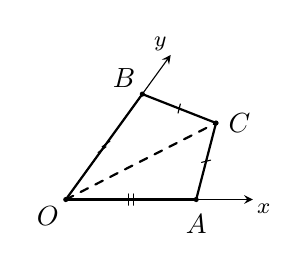
\begin{tikzpicture}[scale=0.72, >=stealth, line join=round, line cap=round]
  \coordinate (O) at (0, 0);
  \coordinate (X) at (3.3, 0);
  \coordinate (Y) at (1.85, 2.55);
  \coordinate (A) at (2.3, 0);
  \coordinate (B) at (1.35, 1.86);
  \coordinate (C) at (2.65, 1.35);

  % Tia Ox, Oy
  \draw[->] (O) -- (X) node[below right=-2pt] {\footnotesize $x$};
  \draw[->] (O) -- (Y) node[above left=-2pt] {\footnotesize $y$};

  % Cac doan thang
  \draw[thick] (O) -- (A);
  \draw[thick] (O) -- (B);
  \draw[thick] (A) -- (C);
  \draw[thick] (B) -- (C);
  \draw[thick, dashed] (O) -- (C);

  % Vach danh dau bang nhau OA = OB (2 vach cat ngang)
  \draw (1.1, -0.1) -- (1.1, 0.1);
  \draw (1.2, -0.1) -- (1.2, 0.1);
  \draw (0.64 - 0.07, 0.88 - 0.05) -- (0.64 + 0.07, 0.88 + 0.05);
  \draw (0.71 - 0.07, 0.98 - 0.05) -- (0.71 + 0.07, 0.98 + 0.05);

  % Vach danh dau bang nhau AC = BC (1 vach cat ngang)
  \draw (2.475 - 0.08, 0.675 - 0.02) -- (2.475 + 0.08, 0.675 + 0.02);
  \draw (2.0 - 0.02, 1.605 - 0.08) -- (2.0 + 0.02, 1.605 + 0.08);

  % Cac diem va nhan
  \fill (O) circle (1.3pt) node[below left=-1pt] {$O$};
  \fill (A) circle (1.3pt) node[below=2pt] {$A$};
  \fill (B) circle (1.3pt) node[above left=-1pt] {$B$};
  \fill (C) circle (1.3pt) node[right=1pt] {$C$};
\end{tikzpicture}
\end{minipage}\par
\vspace{0.4mm}
\noindent\textit{Bài giải:}\dongkeHaiCot{10}
\\ \hline
\end{tabularx}

\vspace{1.5mm}

\noindent
\begin{tabularx}{\linewidth}{|X|}
\hline
\vspace{0.5mm}
\textbf{Câu 14 (0,5 điểm).} Tìm giá trị nhỏ nhất của biểu thức: $A = |x - 2023| + |x - 25|$.\par
\vspace{0.4mm}
\noindent\textit{Bài giải:}\dongkeHaiCot{6}
\\ \hline
\end{tabularx}
\end{document}
